\begin{frame}
    \frametitle{Objectif.}
    \begin{center}
        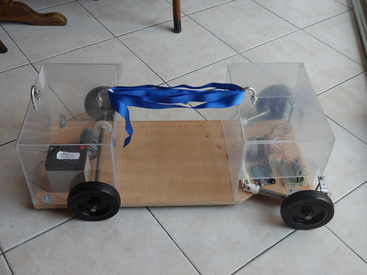
\includegraphics[width=0.95\linewidth]{rcs/intro.png}
    \end{center}
\end{frame}

\begin{frame}
    \frametitle{Chaine de commande.}
    \framesubtitle{Théorique.}
    \only<1-> {
        \begin{block}{Acquérir.}
            \begin{itemize}
                \item Caméra.
            \end{itemize}
        \end{block}
    }
    \only<2-> {
        \begin{block}{Traiter.}
            \begin{itemize}
                \item PandaBoard.
                \item Arduino.
            \end{itemize}
        \end{block}
    }
    \only<3-> {
        \begin{block}{Communiquer.}
            \begin{itemize}
                \item Shield BlueTooth.
                \item Smartphone.
            \end{itemize}
        \end{block}
    }
\end{frame}

\begin{frame}
    \frametitle{Chaine de commande.}
    \framesubtitle{Pratique.}
    \input cmd_log.tex
\end{frame}

